\subsection{ИП, вспомнить всё!}

\begin{enumerate}

  \item Сфорулируйте теорему о трёх перпендикулярах и обратную к ней. Нарисуйте картинку.

  \item Для матрицы
$
  A=\begin{pmatrix}
  4 & 5  \\
  5 & 4  \\
  \end{pmatrix}
$

  \begin{enumerate}
  \item Найдите собственные числа и собственные векторы матрицы;
  \item Найдите определитель $\det A$ и след $\tr A$;
 \item Известно, что $B = A^{-1} + 2018I$, где $I$ — единичная матрица.
 Найдите собственные числа $B$, определитель $\det B$ и след $\tr B$.

  \end{enumerate}


  \item Блондинка Маша встретила 100 динозавров.
  Средний рост динозавров оказался равен 20 метров, а выборочное стандартное отклонение — 5 метров.

  \begin{enumerate}
    \item Постройте 95\% доверительный интервал для математического ожидания роста динозавра.
    \item На уровне значимости 1\% проверьте гипотезу о том, что математическое ожидание
    роста равно 22 метрам. Против альтернативной гипотезе о неравенстве.
    \item Укажите $P$-значение для теста в предыдущем пункте.
  \end{enumerate}

 \item На брег выходят один за одним 33 богатыря. Двадцать вторым по счёту выходит
 богатырь Мефодий. Какова вероятность того, что Мефодий окажется вторым по силе из всех богатырей,
   если известно, что он самый сильный из всех вышедших до него?

\end{enumerate}


\subsection{Вспомнить всё, ответы}

\begin{enumerate}
\item[2.]
\begin{enumerate}
  \item $\lambda^A_1 = -1$, $\lambda^A_2 = 9$,
  $h_1 = \begin{pmatrix}
  1 & -1
  \end{pmatrix}^T$,
  $h_2 = \begin{pmatrix}
  1 & 1
  \end{pmatrix}^T$
  \item $\det(A) = \lambda^A_1 \cdot \lambda^A_2 = -9$, $\tr(A) = \lambda^A_1 +
  \lambda^A_2 = 8$
  \item $\lambda^B_1 = 1 / \lambda^A_1 + 2018 = 2017$,
  $\lambda^B_2 = 1 / \lambda^A_2 + 2018 = 2018 + 1/9$,
  $\det(B) = \lambda^B_1 \cdot \lambda^B_2 = 2017 \cdot (2018 + 1/9)$,
  $\tr(B) = \lambda^B_1 + \lambda^B_2 = 4035 + 1/9$
\end{enumerate}
\item[3.]
\begin{enumerate}
\item $\left[20 - 1.96 \cdot 5 / \sqrt{100}; 20 + 1.96 \cdot 5 / \sqrt{100} \right]$
\item $z_{obs} = -4$, $z_{crit} = \pm 2.6$, основная гипотеза отвергается
\item $p-value \approx 0 $
\end{enumerate}
\item[4.] Заметим, что неважно, каким идёт Мефодий, а главное, что он самый сильный из
$22$ вышедших. Из $22$ вышедших всё равно есть кто-то самый сильный, и если его
считать Мефодием, то ничего не изменится. Значит, нам нужна вероятность того,
что второй лучший из всех попадёт на $22$ места из $33$, а самый лучший на $11$
мест из $32$ оставшихся. Искомая вероятность — $11/48$.

Или по формуле условной вероятности. Пусть $A$ означает, что Мефодий второй по силе
из всех, а $B$ — что он первый по силе из вышедших. Тогда
\[
\P(B) = 1/22,
\]
так как Мефодий должен быть самым сильным из вышедших, и
\[
\P(A \cap B) = 11/33 \cdot 1/32,
\]
так как на $22$-ом месте должен быть самый сильный из вышедших и второй по силе из
всех. Если он второй по силе из вышедших, то первый оказался среди $11$ невышедших,
и эта вероятность равна $11/33$, а вероятность быть вторым по силе среди всех равна
$1/32$. Итого,
\[
\P(A|B) = \frac{\P(A \cap B)}{\P(B)} = \frac{11}{48}.
\]
\end{enumerate}



\subsection{Задачи миниконтрольных ИП}

\begin{enumerate}
  \item Найдите SVD-разложение матрицы $
  \begin{pmatrix}
  2 & 0 & -1 \\
  2 & 1 & 0 \\
  \end{pmatrix}$
 \item Найдите дифференциал $d \cos(r^TAr+br)$, где $A^T=A$ и $b$ — это константы.
 \item Постройте регрессию вектора $y = (4,2,-2)^T$ на вектора $x=(1,0,-1)^T$ и $z=(1,1,-1)^T$
 без константы.
 \item Известно, что $y=x + 2z$. Винни-Пух построил регрессию $\hat y_i = \hat\beta_1 + 0.16 x_i$.
 Пятачок построил регрессию $\hat x_i = \hat \alpha_1 + 1\cdot y_i$.

 Помогите Сове найти коэффициент $\hat \gamma_2$ в регрессии $\hat y_i = \hat\gamma_1 + \hat\gamma_2 z_i$.


\item Величины $U_1$ и $U_2$ независимы и равномерны $U[0;1]$. Рассмотрим пару величин $Y_1 = R\cdot \cos \alpha$, $Y_2 = R\cdot \sin \alpha$, где $R=\sqrt{-2\ln U_1}$, а $\alpha = 2\pi U_2$.
\begin{enumerate}
  \item Выпишите дифференциальную форму для пары $U_1$, $U_2$;
  \item Выпишите дифференциальную форму для пары $Y_1$, $Y_2$;
  \item  Найдите совместный закон распределения $Y_1$ и $Y_2$;
  \item Верно ли, что $Y_1$ и $Y_2$ независимы?
  \item  Как распределены $Y_1$ и $Y_2$ по отдельности?

\end{enumerate}

 \item Спроецируйте вектор $y=(y_1, y_2, y_3, y_4, y_5)'$ на линейную оболочку векторов
 $a=(1, 0, 1,1, 1)'$, $b=(2,1,1,1,1)'$ и $c=(0,3,1,1,1)'$. Выпишите явно квадрат длины
 проекции. Как распределён квадрат длины проекции, если компоненты вектора $y$
 независимы и стандартно нормально распределены.

 \item Докажите эффективность МНК-оценок в задаче множественной регрессии.


\end{enumerate}


\subsection{Контрольная работа-1. Базовая часть}


\begin{question}
Рассмотрим модель множественной регрессии \(Y=X\beta+\varepsilon\), где
\(\hat Y = X\hat\beta\), \(e=Y-\hat Y\). Величина \(RSS\) --- это
квадрат длины вектора
\begin{answerlist}
  \item \(\hat Y - \bar Y\)
  \item \(e\)
  \item \(\varepsilon\)
  \item \(\hat Y\)
  \item \(Y-\bar Y\)
\end{answerlist}
\end{question}




\begin{question}
Крокодил Гена оценивает модель регрессии
\(Y_i = \beta_0 + \beta_1 X_i + \varepsilon_i\) с помощью МНК. Чебурашка
получит такую же оценку коэффициента \(\beta_1\), если будет
минимизировать
\begin{answerlist}
  \item выборочную дисперсию объясняющей переменной
  \item коэффициент детерминации
  \item выборочную ковариацию регрессора и объясняемой переменной
  \item выборочную дисперсию объясняемой переменной
  \item выборочную дисперсию остатков
\end{answerlist}
\end{question}




\begin{question}
Чебурашка оценил модель \(Y_i = \beta_0 + \beta_1 X_i + \varepsilon_i\),
а Крокодил Гена --- модель \(X_i = \gamma_0 + \gamma_1 Y_i + u_i\).
Оказалось, что \(\hat\gamma_1 = 0.25/\hat\beta_1\). Величина \(R^2\) в
регрессии Чебурашки равна
\begin{answerlist}
  \item \(1\)
  \item \(0\)
  \item \(0.75\)
  \item \(0.5\)
  \item \(0.25\)
\end{answerlist}
\end{question}

\begin{solution}
\(R^2 = \hat\beta_1 \cdot \hat\gamma_1\)
\end{solution}



\begin{question}
В модели \(Y_i = \beta_0 + \beta_1 X_i + \varepsilon_i\) при выполненных
предпосылках теоремы Гаусса-Маркова и нормальных ошибках тестовая
статистика \((\hat\beta_1 - \beta_1)/se(\hat\beta_1)\) имеет
распределение
\begin{answerlist}
  \item \(t_{n-2}\)
  \item \(\cN(0;1)\)
  \item \(\chi^2_{n-2}\)
  \item \(\chi^2_1\)
  \item \(\cN(0;\sigma^2)\)
\end{answerlist}
\end{question}




\begin{question}
Крокодил Гена оценил с помощью МНК зависимость
\(Y_i = \beta_0 + \beta_1 X_i + \varepsilon_i\). Оказалось, что
\(\hat \beta_0 = 90\), а \(\hat\beta_1 = 3\). Чебурашка увеличил
переменные \(X\) и \(Y\) на 10\% и снова оценил уравнение регрессии. В
результате этой корректировки
\begin{answerlist}
  \item оценка \(\hat\beta_0\) увеличилась, а оценка \(\hat\beta_1\) не
изменилась
  \item оценки \(\hat\beta_0\) и \(\hat\beta_1\) не изменились
  \item оценки \(\hat\beta_0\) и \(\hat\beta_1\) увеличились
  \item оценки \(\hat\beta_0\) и \(\hat\beta_1\) уменьшились
  \item оценка \(\hat\beta_0\) уменьшилась, а оценка \(\hat\beta_1\) не
изменилась
\end{answerlist}
\end{question}




\begin{question}
В модели парной линейной регрессии со свободным членом
\(Y_i = \beta_0 + \beta_1 X_i + \varepsilon_i\) несмещённой оценкой
дисперсии оценки МНК \(\hat\beta_1\) является
\begin{answerlist}
  \item \(\sum (Y_i - \bar Y)^2 / (n-1)\)
  \item \(RSS/n\)
  \item \(RSS/(n-2)\)
  \item \(RSS/((n-2)\sum_i (X_i - \bar X)^2)\)
  \item \(\sum (Y_i - \bar Y)^2 / (n-2)\)
\end{answerlist}
\end{question}




\begin{question}
Храбрый исследователь Вениамин оценил регрессию
\(\hat Y_i = \underset{(5)}{23} + \underset{(2)}{10}X_i\), в скобках
приведены стандартные ошибки. Доверительный интервал для свободного
члена равен \([14; 32]\). Доверительный интервал для коэффициента
наклона при том же уровне доверия будет равен
\begin{answerlist}
  \item \([6.08; 13.92]\)
  \item \([6; 14]\)
  \item \([5; 15]\)
  \item \([1; 19]\)
  \item \([6.4; 13.6]\)
\end{answerlist}
\end{question}




\begin{question}
По 20 наблюдениям Чебурашка оценил модель
\(Y_i = \beta_0 + \beta_1 X_i + \varepsilon_i\). Известно, что
\(\sum X_i = -10\), \(\sum X_i^2 = 40\), \(\sum X_i Y_i = 10\),
\(\sum Y_i = 50\).

Сумма оценок МНК коэффициентов \(\hat \beta_0 + \hat \beta_1\) равна
\begin{answerlist}
  \item \(4\)
  \item \(5\)
  \item \(3\)
  \item \(2\)
  \item \(1\)
\end{answerlist}
\end{question}

\begin{solution}
========
\end{solution}



\begin{question}
Распределение случайной величины \(X\) задано таблицей

\begin{center}
\begin{tabular}{ccccc}
\toprule
$x$ & 0 & 1 & 2 & 3 \\ 
$\P(X=x)$ & $-b$ & $0.5-b$ & $0.5+b$ & $b$ \\
\bottomrule
\end{tabular}
\end{center}

Вероятность \(\P(X=1)\) равна
\begin{answerlist}
  \item \(0.2\)
  \item \(0.4\)
  \item \(0.5\)
  \item \(0\)
  \item \(0.3\)
\end{answerlist}
\end{question}




\begin{question}
Оценки МНК вектора коэффициентов регрессии \(Y=X\beta + \varepsilon\)
находятся по формуле
\begin{answerlist}
  \item \((XX')^{-1}X'Y\)
  \item \(X'Y(X'X)^{-1}\)
  \item \((X'X)^{-1}X'Y\)
  \item \((X'X)^{-1}YX\)
  \item \((XX')^{-1}Y'X\)
\end{answerlist}
\end{question}

\begin{solution}
========
\end{solution}




\begin{enumerate}
  \item (5 баллов) Случайные величины $X$ и $Y$ независимы и имеют хи-квадрат распределение
  с 5 и с 10 степенями свободы, соответственно. Случайная величина $Z$ равна $Z = (X+Y)/X$.

  Найдите значение $z^*$ такое, что $\P(Z > z^*)=0.05$.
  \item (5 баллов) Докажите, что для модели парной регрессии $Y_i = \beta_0 + \beta_1 X_i + \varepsilon_i$,
оцененной с помощью МНК, выполнено равенство $\sum_{i=1}^n Y_i = \sum_{i=1}^n \hat Y_i$.

  \item (5 баллов) Аккуратно сформулируйте теорему Гаусса-Маркова для случая парной регрессии.

  \item (10 баллов) На основании 62 наблюдений Чебурашка оценил функцию спроса на апельсины:

 \[
 \hat Y_i = \underset{(1.6)}{3} - \underset{(0.2)}{1.25} X_i, \text{ где } \sum_i (X_i - \bar X)^2 =2.25
 \]

 В скобках приведены стандартные ошибки коэффициентов, случайные ошибки в регрессии можно считать нормальными.


  \begin{enumerate}
    \item Проверьте гипотезы о значимости каждого из коэффициентов регрессии при уровне значимости 5\%.
    \item Проверьте гипотезу о равенстве коэффициента наклона -1 при уровне значимости 5\%
    и односторонней альтернативной гипотезе, что коэффициент наклона меньше -1.
    \item Найдите оценку дисперсии ошибок.
    \item Найдите 95\% интервальный индивидуальный прогноз в точке $X=8$.
  \end{enumerate}
\end{enumerate}

\subsection{Контрольная работа-1. Базовая часть, решения}

\begin{enumerate}
\item Распишем вероятность $\P(Z >z^*)$:
\begin{align*}
\P(Z >z^*) &= \P \left(\frac{X+Y}{X} > z^* \right) = \P \left(1 + \frac{Y}{X} > z^* \right) \\
&= 1 - \P\left(\frac{Y}{X} \leq z^* - 1 \right) = 1 - \P\left(\frac{Y/10}{X/5} \leq \left(z^* - 1\right) \cdot \frac{5}{10} \right)
\end{align*}
Заметим, что
\[
W = \frac{Y/10}{X/5} \sim F_{10,5}
\]
Подставив случайную величину $W$ в выражение для $\P(Z >z^*)$, получим:
\[
\P\left(W \leq 0.5(z^* - 1) \right) = 0.95 \Rightarrow 0.5(z^* - 1) = 4.74 \Rightarrow z^* = 10.48
\]
\item Запишем $Y_i$ через оценку $\hat Y_i$ и остатки $e_i = Y_i - \hat Y_i$ и
просуммируем обе части выражения:
\begin{align*}
Y_i &= \hat Y_i + e_i \\
\sum_{i=1}^n Y_i &= \sum_{i=1}^n \hat Y_i + \sum_{i=1}^n e_i
\end{align*}
Нужно показать, что последнее слагаемое в полученном равенстве равно нулю:
\[
\sum_{i=1}^n e_i = \sum_{i=1}^n Y_i - n\hb_0 - \hb_1 \sum_{i=1}^n X_i
\]
Разделим обе части на $n$:
\[
\frac{1}{n} \sum_{i=1}^n e_i = \bar Y - \hb_0 - \hb_1 \bar X
\]
Осталось вспомнить, что $\hb_0 = \bar Y - \hb_1 \bar X$.
\item Если для модели $Y_i = \beta_0 + \beta_1 X_i + \varepsilon_i, i=1, \ldots, n$
выполнены условия о том, что
\begin{enumerate}
  \item модель правильно специфицирована,
  \item $X_i$ являются детерминированными величинами и не равны между собой,
  \item $\E(\varepsilon_i) = 0 \quad \forall i$,
  \item $\Var(\varepsilon_i) = \sigma^2_{\varepsilon} \quad \forall i$,
  \item $\Cov(\varepsilon_i, \varepsilon_j) = 0 \quad \forall i \neq j$,
\end{enumerate}
то МНК-оценки $\hb_0$, $\hb_1$ являются лучшими линейными несмещёнными оценками.
\item
\begin{enumerate}
\item Для проверки гипотезы о значимости отдельного коэффициента используем $t$-тест:
\[
t_{obs} = \frac{\hb - \beta}{\hat{\sigma}_{\hb}} \sim t_{n-k}
\]
\begin{itemize}
\item для $\beta_0$: $t_{obs} = 1 / 1.6 = 0.625 < 2 = t_{crit} \Rightarrow$
нет оснований отвергать $H_0$.
\item для $\beta_1$: $t_{obs} = -1.25 / 0.2 = 6.25 > 2 = t_{crit} \Rightarrow$
$H_0$ отвергается.
\end{itemize}
\item Необходимо проверить следующую гипотезу:
\[
\begin{cases}
H_0: \beta_1 = -1 \\
H_a: \beta_1 < -1
\end{cases}
\]
Проверяем:
\[
t_{obs} = \frac{-1.25 - (-1)}{0.2} = -1.25 > -1.67 = t_{crit}
\]
Нет оснований отвергать нулевую гипотезу.
\item Из соотношения для оценки дисперсии $\hb_1$ получим:
\begin{align*}
\hat{\sigma}^2_{\hb_1} &= \frac{\hat{\sigma}^2_{\varepsilon}}{\sum_{i=1}^{62}(X_i - \bar X)^2} \Rightarrow \\
\hat{\sigma}^2_{\varepsilon} &= \hat{\sigma}^2_{\hb_1} \cdot \sum_{i=1}^{62}(X_i - \bar X)^2 \\
&= (0.2)^2 \cdot 2.25 = 0.09
\end{align*}
\item Найдём точечный прогноз в точке $X = 8$:
\[
\hat Y_f = 3 - 1.25 \cdot 8 = -7
\]
Найдём оценку дисперсии прогноза:
\begin{align*}
\widehat{\Var}(\hat Y_f) &= \widehat{\Var} \left(\hb_0 + \hb_1 \cdot 8 \right) \\
&= \widehat{\Var} \left(\hb_0\right) + 64 \widehat{\Var} \left(\hb_1 \right) + 2 \cdot 8 \widehat{\Cov}(\hb_0, \hb_1) \\
&= 1.6^2 + 64 \cdot 0.2^2 + 16 \cdot \frac{-\bar X \hat{\sigma}^2_{\varepsilon}}{\sum_{i=1}^{62}\left(X_i - \bar X\right)^2} \\
&= 1.6^2 + 64 \cdot 0.04 - 16 \cdot \frac{\sqrt{3.96} \cdot 0.09}{2.25} \\
&\approx 3.9
\end{align*}
Осталось выписать доверительный интервал:
\[
\left[-7 -2 \cdot \sqrt{3.9}; -7 + 2 \cdot \sqrt{3.9} \right]
\]
\end{enumerate}
\end{enumerate}


\subsection{Контрольная работа-1. ИП часть}

\begin{enumerate}
  \item Храбрый исследователь Вениамин поделил выборку на обучающую $(X, y)$ и тестовую $(X_{test}, y_{test})$.
  Регрессоры $X$ и $X_{test}$ Вениамин считает нестохастическими, а предпосылки
  теоремы Гаусса-Маркова — выполненными на всей исходной выборке. Естественно,
  $\hat y_{test} = X_{test}\hat\beta$, где $\hat\beta$ оценивается по обучающей выборке.

  Помогите Вениамину найти $\Var(\hat y_{test})$ и $\Cov(\hat \beta, \hat y_{test})$.

  \item Рассмотрим матрицу $X$ полного ранга с $n$ наблюдениями и $k$ столбцами.
  В каких границах могут лежать диагональные элементы матрицы-шляпницы $H$?
  Чему равно их среднее значение?

  Подсказка: найдите $\Var(\hat y)$ и $\Var(\hat u)$ в рамках предпосылок теоремы Гаусса-Маркова.

  \item Рассмотрим стандартный $t$-тест на равенство некоторого коэффициента бета нулю.
  Докажите, что
  \[
         t^2 = \frac{RSS_r - RSS_{ur}}{RSS_{ur}/(n-k)},
  \]
  где $RSS_r$ — сумма квадратов остатков в модели без тестируемого коэффициента
  (выкинут регрессор при проверямом коэффициенте),
  $RSS_{ur}$ — аналогичная сумма в модели с включённым тестируемым коэффициентом, $k$ —
  число оцениваемых коэффициентов бета в модели с тестируемым коэффициентом, $n$ —
  количество наблюдений.

  Утешительный приз: упростите эту формулу для случая парной регрессии и докажите её :)

  \item Рассмотрим стандартную ошибку оценки коэффициента бета при регрессоре $z$
  в множественной регрессии.
  Докажите, что

  \[
         se^2(\hat\beta_z) = \frac{RSS / (n-k)}{\sum (z_i - \bar z)^2} \cdot \frac{1}{1 - R^2_z},
  \]
  где $R^2_z$ — коэффициент детерминации во вспомогательной регресии объясняющей переменной
  $z$ на остальные объясняющие переменные.

  Утешительный приз: упростите эту формулу для случая парной регрессии и докажите её :)


   \item У Винни-Пуха есть случайный вектор $w$ и одномерная случайную величину $z$.
   Винни-Пуху известны величины $\Cov(w, w) = A$ и $\Cov(w, z) = b$.

   К сожалению, у Винни-Пуха опилки в голове, а он очень хочет найти такую линейную комбинацию
   компонент вектора $w$, которая была бы сильнее всего коррелирована со случайной
   величиной $z$.

   Помогите Винни-Пуху!

   Как выглядят веса этой линейной комбинации?
   Чему равна максимально возможная корреляция?

 \item Машенька построила парную регрессию по 11 наблюдениям с $R^2=
0.95$. Чтобы напакостить Машеньке, Вовочка переставил в случайном
порядке значения зависимой переменной и предложил Машеньке заново оценить модель.

Какой ожидаемый $R^2$ получит Машенька?
\end{enumerate}


\subsection{ИП-часть, решения}
\begin{enumerate}
\item Дисперсия:

\begin{align*}
\Var \left(\hat{y}_{test}\right) &= \Var \left(X_{test} \hat\beta \right) \\
&= X_{test} \Var\left((X'X)^{-1} X' y \right) X'_{test} \\
&= X_{test} (X'X)^{-1} X' \sigma^2 \cdot I X (X'X)^{-1}  X'_{test} \\
&= \sigma^2 X_{test} (X'X)^{-1} X'_{test}
\end{align*}

Ковариация:
\begin{align*}
\Cov\left(\hat \beta, \hat{y}_{test}\right) &= \Cov\left(\hat \beta,  X_{test} \hat{\beta} \right) \\
&= \Var\left(\hat \beta\right) X'_{test} \\
&= \Var\left((X'X)^{-1} X' y \right)X'_{test} \\
&= (X'X)^{-1} X' \sigma^2 \cdot I X (X'X)^{-1}  X'_{test} \\
&= \sigma^2 (X'X)^{-1} X'_{test}
\end{align*}

\item
Воспользуемся подсказкой и найдём:
\begin{align*}
\Var\left(\hat y\right) &= \Var \left(Hy \right) = H \Var(y) H' = \sigma^2 H \\
\Var \left(\hat u \right) &= \Var \left(y - \hat y\right) = \Var \left((I-H)y\right) = \sigma^2 (I-H)
\end{align*}


Соответственно, для диагональных элементов выполнятются соотношения:
\[
\Var\left(\hat y_i \right) = \sigma^2 h_{ii} \text{ и } \Var \left(\hat u_i \right) = \sigma^2(1 - h_{ii}),
\]
откуда следует, что диагональные элементы матрицы-шляпницы лежат в пределах от $0$ до $1$.

Вспомним, что сумму диагональных элементов, или след матрицы, можно вычислить
как сумму её собственных значений.
Поскольку матрица-шляпница является проектором, её собственные числа равны либо
 $0$, либо $1$.
Это легко показать. Пусть $\lambda$ — собственное значение матрицы $H$ с собственным
вектором $v$. Для $H$ выполняется соотношение $H^2 = H$, а значит верно и
\[
\lambda^2 v = H^2 v = H v = \lambda v,
\]
где $v \neq 0$. Отсюда получаем уравнение $\lambda^2 = \lambda$, корни которого —
$0$ и $1$.

Осталось заметить, что для собственных чисел $\lambda = 1$ собственные вектора
лежат в $Lin(X)$, а для нулевых собственных чисел — перпендикулярны ей.
Значит, количество единиц совпадает с размерностью пространства, на которое проецируем.
В нашем случае оно равно $k$. Значит, среднее диагональных элементов — $k/n$.

\item Утверждение можно доказать геометрически.

\begin{align*}
\frac{t}{\sqrt{n-2}} &=
\frac{\hat \beta_2}{\sqrt{n-2}se\left(\hat\beta_2\right)} =
\frac{\hat \beta_2}{\sqrt{n-2}\frac{\hat \sigma}{\sqrt{\sum\limits_{i=1}^n (x_i - \bar x)^2}}}
= \frac{\hat \beta_2 \sqrt{\sum\limits_{i=1}^n (x_i - \bar x)^2}}{\sqrt{n-2}\frac{\sqrt{\sum\limits_{i=1}^n (y_i - \hat y_i)^2}}{\sqrt{n-2}}} \\
&= \frac{\hat \beta_2 \lVert x^c \rVert}{\sqrt{RSS}} = \ctg \varphi\\
\end{align*}

\begin{figure}[ht!]
\begin{center}
\subfigure[]{
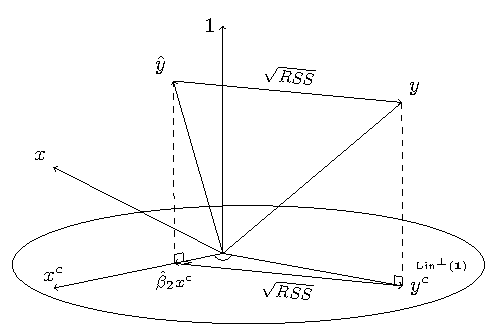
\includegraphics[width=0.35\linewidth]{figures/04_ttest.pdf}
\label{fig:ttest_3d}}
%\hspace{4ex}
\subfigure[]{
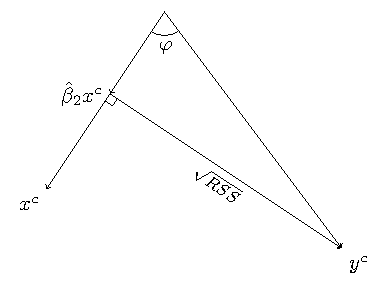
\includegraphics[width=0.35\linewidth]{figures/04_ttest_lin.pdf}
\label{fig:ttest_lin}}
\caption{\subref{fig:ttest_3d}: Регрессия $y$ на $\Lin(x, \mathbf{1})$ и соответствующие проекции;
\subref{fig:ttest_lin}: $\Lin^{\perp}(\mathbf{1})$.}
\end{center}
\end{figure}

\[
F = \frac{(RSS_{R} - RSS_{UR})/q}{RSS_{UR}/(n-k_{UR})} =
\ctg^2 \varphi \cdot \frac{n - k_{UR}}{q}
\]

\begin{figure}[ht!]
\centering
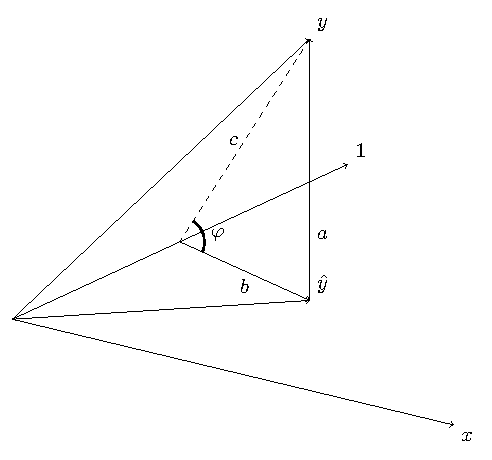
\includegraphics[scale=0.55]{figures/04_ftest.pdf}
\caption{F-статистика пропорциональна квадрату котангенса $\varphi$,
где $a$ означает $\sqrt{RSS_{UR}}$, $b$ — $\sqrt{RSS_{R} -RSS_{UR}}$,
$c$ — $\sqrt{RSS_{R}}$.}
\label{fig:ftest}
\end{figure}

В случае парной регрессии $k_{UR} = 2, q = 1$.

\item Представим матрицу регрессоров в виде двух блоков: $X = [Z \quad W]$, где $Z$ —
это регрессор (вектор), для которого мы будем искать стандартную ошибку, а
$W$ — это матрица всех остальных регрессоров.
Известно, что
\[
\Var\left(\hat{\beta}_{Z} \right) = \sigma^2 (X'X)^{-1}_{11},
\]
то есть нам нужно найти только первый элемент матрицы $X'X$.
Эта матрица является блочной и в наших обозначениях имеет вид:
\[
X'X = \begin{pmatrix}
Z'Z & Z'W \\
W'Z & W'W
\end{pmatrix}
\]

Чтобы найти обратную матрицу в общем случае, нужно решить систему:
\[
\begin{pmatrix}
A & B \\
C & D
\end{pmatrix}
\cdot
\begin{pmatrix}
E & F \\
G & H
\end{pmatrix}
=
\begin{pmatrix}
I & 0 \\
0 & I
\end{pmatrix},
\]
где матрица слева изветсна, матрица из блоков $E, F, G, H$ является обратной к ней.
Решая эту систему, например, методом Гаусса, получим:
\[
E = (A-BD^{-1}C)^{-1},
\]
а остальные элементы нас не интересуют.
Возвращаясь к нашим обозначениям, запишем:
\[
(X'X)^{-1}_{11} = \left(Z'Z - Z'W \left(W'W \right)^{-1} W'Z \right)
\]
Обозначив $\left(W'W \right)^{-1} W'= H$ (проектор во вспомогательной регрессии на все
переменные, кроме Z), упростим полученное выражение:
\[
(X'X)^{-1}_{11} = Z'(I-H)Z
\]
Как промежуточный итог мы получили:
\[
\Var\left(\hat{\beta}_{Z} \right) = \frac{\sigma^2}{Z'(I-H)Z}
\]
Теперь рассмотрим коэффициент детерминации во вспомогательной регрессии:
\[
1 - R^2_Z = \frac{RSS_Z}{TSS_Z} = \frac{(Z - \hat Z)'(Z - \hat Z)}{(Z - \bar Z)'(Z - \bar Z)} = \frac{((I-H)Z)'(I-H)Z}{(Z - \bar Z)'(Z - \bar Z)}
= \frac{Z'(I-H)Z}{(Z - \bar Z)'(Z - \bar Z)}
\]
Выражая отсюда числетель, получаем:
\[
Z'(I-H)Z = \left( 1 - R^2_Z \right) \cdot \sum (Z_i - \bar Z)^2
\]
Осталось вспомнить оценку для $\sigma^2$ и записать финальный резульат:
\[
\widehat{\Var}\left(\hat{\beta}_{Z} \right) = \frac{RSS/(n-k)}{\sum (Z_i - \bar Z)^2} \cdot \frac{1}{1 - R^2_Z}
\]

\item В том виде, в котором задача дана, она не решается.
Однако можно было выписать целевую функцию и взять её дифференциал:
\[
\Corr(\alpha^T w, z) = \frac{\Cov(\alpha^T w, z)}{\sqrt{\Var(\alpha^T w)\Var(z)}}
= \frac{\alpha^T \Cov(w,z)}{\sqrt{\alpha^T\Var(w) \alpha \Var(z)}} \to \max_{\alpha}
\]
Также можно было заметить, что эта задача напоминает МНК.
Пусть $\hat z$ — проекция $z$ на $\Lin(w_1, \ldots, w_k)$,
а $\tilde{z}$ — произвольный вектор из $\Lin(w_1, \ldots, w_k)$.
Обозначив угол между $z$ и $\hat z$ за $\alpha$, между $z$ и $\tilde z$ за $\beta$,
можем записать:
\[
\Corr(z, \hat z) = \cos \alpha \geq \cos \beta = \Corr(z, \tilde z)
\]
при $\alpha \leq \beta \leq 90^{\circ}$.
И задача максимизации $\Corr(z, \tilde z)$ будет эквивалентна задаче МНК.

\item Без ограничения общности центрируем исходные переменные.
Значения регрессора обозначим $x_i$, исходную зависимую переменную $\tilde{y}_i$,
а переставленную в случайном порядке $y_i$.
По условию, $\sum y_i^2 = \sum \tilde{y}_i^2$.

Фиксируем исходные переменные и находим:
\[
\E(R^2 | \tilde{y}) = \E\left( \frac{(\sum x_i y_i )^2}{\sum x_i^2 \sum y_i^2}  \right) =
\frac{\Var\left(\sum x_i y_i | \tilde{y}\right)}{\sum x_i^2 \sum y_i^2}
\]

Для начала найдём дисперсию отдельного игрека:
\[
\Var(y_i | \tilde{y}) = \frac{\sum \tilde{y}_i^2}{n} = \frac{\sum y_i^2}{n}
\]

А теперь из $\Cov(y_1, \sum y_i | \tilde{y}) =0$ найдём и дисперсию нужной суммы:
\[
\Var\left(\sum x_i y_i | \tilde{y}\right) =
\Var(y_i | \tilde{y}) \left(  \sum x_i^2 - \sum_{i\neq j} x_i x_j \frac{1}{n-1}  \right) =
\Var(y_i | \tilde{y}) \frac{n}{n-1} \sum x_i^2 = \frac{\sum x_i^2 \sum y_i^2 }{n-1}
\]

Заканчиваем подсчёт,
\[
\E(R^2 | \tilde{y}) = \frac{1}{n-1}
\]

Следовательно, и $\E(R^2) = \frac{1}{n-1} = 0.1$.

\end{enumerate}


\subsection{Контрольная работа 2. 26-12-2018}

\subsection*{Тест}


\begin{question}
(1 балл) Исследователь Феофан оценил с помощью МНК модель
\(Y = \beta_0 I + \beta_1 Z + \beta_2 W + u\), где \(I\) — столбец из
единиц. Для матрицы факторов, \(X = (I Z W)\), известно, что \[
(X'X)^{-1} = \begin{pmatrix}
0.04 & 0.012 & -0.008 \\
0.012 & 0.03 & -0.007 \\
-0.008 & -0.007 & 0.02
\end{pmatrix}
\] Предпосылки теоремы Гаусса-Маркова выполнены. Отношение дисперсии
оценки \(\hat \beta_0\) к дисперсии оценки \(\hat \beta_2\) равно
\begin{answerlist}
  \item \(2\)
  \item \(-5/1\)
  \item \(10/3\)
  \item \(1/2\)
  \item \(3/2\)
  \item нет верного ответа
\end{answerlist}
\end{question}

\begin{solution}
\begin{answerlist}
  \item Good answer :)
  \item Bad answer :(
  \item Bad answer :(
  \item Bad answer :(
  \item Bad answer :(
\end{answerlist}
\end{solution}


\begin{question}
(2 балла) Исследовательница Клеопатра оценила модель
\(\ln Y_i = \beta_0 + \beta_1 \ln X_i + \beta_2 \ln Z_i + \beta_3 \ln W_i + u_i\).
Клеопатра хочет протестировать гипотезу \(H_0\):
\(\beta_3 + 2\beta_1 = 1\). Для этой цели можно оценить вспомогательную
регрессию
\begin{answerlist}[2]
  \item \(\ln(Y_i \cdot W_i) = \gamma_0 + \gamma_1 \ln (X_i \cdot W_i^2) + \gamma_2 \ln Z_i + u_i\)
  \item \(\ln(Y_i \cdot W_i) = \gamma_0 + \gamma_1 \ln (X_i/W_i^2) + \gamma_2 \ln Z_i + u_i\)
  \item \(\ln(Y_i/W_i) = \gamma_0 + \gamma_1 \ln (X_i \cdot W_i^2) + \gamma_2 \ln Z_i + u_i\)
  \item \(\ln(Y_i/W_i) = \gamma_0 + \gamma_1 \ln(X_i/W_i^2) + \gamma_2 \ln{Z_i} + u_i\)
  \item \(\ln(Y_i/W_i^2) = \gamma_0 + \gamma_1 \ln (X_i/W_i) + \gamma_2 \ln Z_i + u_i\)
  \item нет верного ответа
\end{answerlist}
\end{question}

\begin{solution}
\begin{answerlist}
  \item Bad answer :(
  \item Bad answer :(
  \item Bad answer :(
  \item Good answer :)
  \item Bad answer :(
\end{answerlist}
\end{solution}


\begin{question}
(1 балл) Какое условие НЕ требуется в теореме Гаусса-Маркова?
\begin{answerlist}[2]
  \item матрица регрессоров \(X\) имеет полный ранг
  \item модель \(Y=X\beta + \varepsilon\) правильно специфицирована
  \item случайные ошибки \(\varepsilon_i\) не коррелированы
  \item случайные ошибки \(\varepsilon_i\) имеют одинаковые дисперсии
  \item случайные ошибки \(\varepsilon_i\) нормально распределены
  \item нет верного ответа
\end{answerlist}
\end{question}

\begin{solution}
\begin{answerlist}
  \item Bad answer :(
  \item Bad answer :(
  \item Bad answer :(
  \item Bad answer :(
  \item Good answer :)
\end{answerlist}
\end{solution}


\begin{question}
(1 балл) Выборочная корреляция между регрессорами \(X\) и \(Z\) равна \(0.5\). В
регрессии \(\hat Y_i = \hat\beta_0 + \hat\beta_1 X_i + \hat\beta_2 Z_i\)
показатель \(VIF\) для регрессора \(X\) равен
\begin{answerlist}
  \item \(1/4\)
  \item \(4/3\)
  \item \(1/2\)
  \item \(2\)
  \item \(3/4\)
  \item нет верного ответа
\end{answerlist}
\end{question}

\begin{solution}
\begin{answerlist}
  \item Bad answer :(
  \item Good answer :)
  \item Bad answer :(
  \item Bad answer :(
  \item Bad answer :(
\end{answerlist}
\end{solution}


\begin{question}
(2 балла) Для регрессии
\(\hat Y_i = \hat\beta_0 + \hat\beta_1 X_i + \hat\beta_2 Z_i + \hat\beta_3 W_i\),
оценённой по 24 наблюдениям, \(R^2=0.9\).

При проверке гипотезы о неадекватности модели \(F\)-статистика равна
\begin{answerlist}
  \item \(200.27\)
  \item \(5/9\)
  \item \(45\)
  \item \(189/2\)
  \item \(60\)
  \item нет верного ответа
\end{answerlist}
\end{question}

\begin{solution}
\begin{answerlist}
  \item Bad answer :(
  \item Bad answer :(
  \item Bad answer :(
  \item Bad answer :(
  \item Good answer :)
\end{answerlist}
\end{solution}


\begin{question}
(2 балла) Для регрессионной модели со свободным членом известно, что \[
X'X = \begin{pmatrix}
20 & 0 & 0 \\
0 & 4 & 3 \\
0 & 3 & 5
\end{pmatrix}, \; \;
X'Y = \begin{pmatrix}
40 \\
10 \\
13
\end{pmatrix}, \;\;
\sum_{i=1}^n Y_i^2 = 140.
\] Коэффициент \(R^2\) в этой модели равен
\begin{answerlist}
  \item \(9/35\)
  \item недостаточно информации
  \item \(13/14\)
  \item \(0.5\)
  \item \(0.6\)
  \item нет верного ответа
\end{answerlist}
\end{question}

\begin{solution}
\begin{answerlist}
  \item Bad answer :(
  \item Bad answer :(
  \item Bad answer :(
  \item Bad answer :(
  \item Good answer :)
\end{answerlist}
\end{solution}


\begin{question}
(1 балл) Портос построил регрессию по 66 наблюдениям,
\(\hat Y_i = \hat\beta_0 + \hat\beta_1 X_i + \hat\beta_2 W_i + \hat\beta_3 Z_i\),
\(RSS=140\). Затем Портос оценил вспомогательную регрессию,
\(\hat{\hat {Y}}_i = \hat\gamma_0 + \hat\gamma_1 X_i + \hat\gamma_2 W_i + \hat\gamma_3 Z_i + \hat\delta_2 \hat Y_i^2 + \hat\delta_3 \hat Y_i^3\),
\(RSS=120\).

При проверке гипотезы о правильной спецификации модели в тесте Рамсея
\(F\)-статистика равна
\begin{answerlist}
  \item \(5\)
  \item \(10/3\)
  \item \(6\)
  \item \(30/7\)
  \item \(11/3\)
  \item нет верного ответа
\end{answerlist}
\end{question}

\begin{solution}
\begin{answerlist}
  \item Good answer :)
  \item Bad answer :(
  \item Bad answer :(
  \item Bad answer :(
  \item Bad answer :(
\end{answerlist}
\end{solution}


\begin{question}
(2 балла) Арамис построил регрессию по 66 наблюдениям: \[
\hat Y_i = \underset{(0.4)}{4} + \underset{(5)}{6}X_i + \underset{(2)}{4.4} Z_i - \underset{(2)}{3} Q_i - \underset{(3)}{9} R_i + \underset{(10)}{16} S_i.
\]
В скобках указаны стандартные ошибки.
Показатель \(R^2_{adj}\) \emph{может} увеличиться при удалении из
модели группы факторов
\begin{answerlist}
  \item \(S\)
  \item \(X\), \(Q\)
  \item \(X\), \(S\)
  \item \(X\), \(Q\), \(S\)
  \item \(Q\), \(S\)
  \item нет верного ответа
\end{answerlist}
\end{question}

\begin{solution}
\begin{answerlist}
  \item Bad answer :(
  \item Bad answer :(
  \item Bad answer :(
  \item Good answer :)
  \item Bad answer :(
\end{answerlist}
\end{solution}


\begin{question}
(1 балл) Чудо-швабры производятся на разных заводах по одной из двух технологий,
\(A\) или \(B\). Исследователь оценил две модели зависимости выпуска,
\(Y\), от количества сырья, \(X\), и технологии:

\(\hat Y_i = \hat \alpha_0 + \hat\alpha_1 A_i + \hat\alpha_2 X_i + \hat\alpha_3 A_i X_i\);

\(\hat Y_i = \hat \beta_0 + \hat\beta_1 B_i + \hat\beta_2 X_i + \hat\beta_3 B_i X_i\).

Переменная \(A_i\) равна единице для заводов с технологией \(A\) и нулю
иначе, а переменная \(B_i\) равна единице для заводов с технологией
\(B\) и нулю иначе.

Оценки коэффициентов связаны соотношением
\begin{answerlist}
  \item \(\hat\alpha_1 = \hat\beta_0\)
  \item \(\hat\alpha_0 = \hat\beta_0 + \hat\beta_1\)
  \item \(\hat\alpha_0 = \hat\beta_0\)
  \item \(\hat\alpha_2 = \hat\beta_2\)
  \item \(\hat\alpha_0 + \hat\alpha_1 = \hat\beta_0\)
  \item нет верного ответа
\end{answerlist}
\end{question}

\begin{solution}
\begin{answerlist}
  \item Bad answer :(
  \item Bad answer :(
  \item Bad answer :(
  \item Bad answer :(
  \item Good answer :)
\end{answerlist}
\end{solution}


\begin{question}
(1 балл) Исследовательница Надежда оценила регрессию в отклонениях,
\(\hat y_i = x_i + 2 z_i\) с помощью МНК. Известно, что \(\bar Y=5\),
\(\bar X =6\), \(\bar Z=-2\). В регрессии нецентрированных переменных,
\(\hat Y_i = \hb_0 + \hb_1 X_i + \hb_2 Z_i\), оценка коэффициента
\(\hb_0\) равна
\begin{answerlist}
  \item \(1\)
  \item \(4\)
  \item \(2\)
  \item \(5\)
  \item \(3\)
  \item нет верного ответа
\end{answerlist}
\end{question}

\begin{solution}
\begin{answerlist}
  \item Bad answer :(
  \item Bad answer :(
  \item Bad answer :(
  \item Bad answer :(
  \item Good answer :)
\end{answerlist}
\end{solution}


\subsection*{Задачи}
\begin{enumerate}
\item
(5 баллов)
Рассмотрим алгоритм LASSO с параметром регуляризации $\lambda$
для модели $Y=X\beta + \varepsilon$, где все переменные центрированы.
\begin{enumerate}
    \item Выпишите целевую функцию алгоритма.
    \item Что произойдет с оценками $\hat\beta_{LASSO}$ при $\lambda \to \infty$?
    \item Что произойдет с оценками $\hat\beta_{LASSO}$ при $\lambda \to 0$?
\end{enumerate}
\item
(5 баллов)
По 200 фирмам была оценена зависимость выпуска $Y$ от труда $L$ и капитала $K$
с помощью двух моделей:

Модель Кобба-Дугласа: $\ln{Y_i} = \beta_0 + \beta_1 \ln{L_i} + \beta_2 \ln{K_i} +
\varepsilon_i$

Транслоговая модель: $\ln{Y_i} = \gamma_0 + \gamma_1 \ln{L_i} + \gamma_2 \ln{K_i} +
\gamma_3 (0.5 \ln^2{L_i}) + \gamma_4 (0.5 \ln^2{K_i}) + \gamma_5 \ln{K_i} \ln{L_i} +
\varepsilon_i$

Оценки коэффициентов обеих моделей (в скобках приведены стандартные ошибки):

\begin{tabular}{lcc}
\toprule
Переменная & Модель Кобба-Дугласа & Транслоговая модель \\
\midrule
константа & $1.1706$ ($0.326$) & $0.9441$ ($2.911$)   \\
$\ln L$ & $0.6029$ ($0.125$) & $3.613$ ($1.548$)  \\
$\ln K$ & $0.375$ ($0.085$) & $-1.893$ ($1.016$)  \\
$0.5 \ln^2 L$ &  & $-0.964$ ($0.707$)  \\
$0.5 \ln^2 K$ & & $0.0852$ ($0.2922$) \\
$\ln L \ln K$ & & $0.3123$ ($0.4389$)  \\
$R^2$ & $0.9$ & $0.954$  \\
\bottomrule
\end{tabular}

В модели Кобба-Дугласа $\hCov(\hb_1, \hb_2)= -0.0096$.

На уровне значимости $\alpha = 0.05$ проверьте следующие гипотезы:
\begin{enumerate}
\item В модели Кобба-Дугласа эластичность выпуска по капиталу равна единице.
\item В модели Кобба-Дугласа эластичности выпуска по труду и капиталу одинаковы.
\item В транслоговой модели $\gamma_3 = 0$.
\item В транслоговой модели $\gamma_3 = \gamma_4 = \gamma_5 = 0$.
\end{enumerate}

\item
(4 балла)
Исследователь оценил зависимость продолжительности жизни $Y$ от концентрации
промышленных выбросов в атмосфере $X$ и ежегодных частных расходов на медицинскую
помощь $Z$.

Для $300$ жителей индустриальных центров, $\hat{Y}_i = \underset{(10.43)}{65.91} -
\underset{(0.0001)}{0.03}X_i - \underset{(0.019)}{0.036}Z_i, \; RSS = 300$.

Для $200$ сельских жителей, $\hat{Y}_i = \underset{(15.3)}{58.4} -
\underset{(0.006)}{0.017}X_i - \underset{(0.007)}{0.024}Z_i, \; RSS = 200$.

А также по общей выборке, $\hat{Y}_i = \underset{(12.4)}{63.2} -
\underset{(0.005)}{0.02}X_i - \underset{(0.001)}{0.031}Z_i, \; RSS = 900$.

В скобках приведены стандартные ошибки.

Можно ли считать, что зависимость едина для городских и сельских жителей?
Ответ обоснуйте подходящим тестом, аккуратно выписав тестируемую гипотезу.

\item
(5 баллов)
Исследователь Д'Артаньян стандартизировал (центрировал и нормировал) все
имеющиеся регрессоры и поместил их в столбцы матрицы $\tilde X$. Выборочная
корреляционная матрица регрессоров равна:
\[
\begin{pmatrix}
1 & 0.85 & 0  \\
0.85 & 1 & 0  \\
0 & 0 & 1 \\
\end{pmatrix}.
\]
\begin{enumerate}
    \item Найдите параметр обусловленности (condition number) матрицы
    $\tilde X^T \tilde X$.
    \item Вычислите одну или две главные компоненты, объясняющие не менее
    $70$\% суммарной дисперсии стандартизированных регрессоров. Выпишите
    найденные компоненты как линейные комбинации столбцов матрицы $\tilde X$.
\end{enumerate}

\item
(6 баллов)
Для $400$ голландских магазинов модной одежды с помощью трёх моделей оценили
зависимость продаж в расчете на квадратный метр в гульденах, $Sales$, от:
\begin{itemize}
\item общей площади магазина, $Size$, в м$^2$;
\item количества сотрудников, работающих целый день, $Nfull$;
\item количества временных рабочих, $Ntemp$;
\item дамми-переменной $Owner$, равной единице, если собственник один, и нулю иначе.
\end{itemize}

$\widehat{Sales}_i = \underset{(718)}{6083} - \underset{(1.59)}{15.25}Size_i +
\underset{(171)}{1452.8} Nfull_i + \underset{(423)}{420.15} Ntemp_i -
\underset{(361)}{1464.1} Owner_i$

$\ln \widehat{Sales}_i = \underset{(0.11)}{8.59} - \underset{(0.00024)}{0.0024}Size_i +
\underset{(0.026)}{0.183} Nfull_i + \underset{(0.066)}{0.102} Ntemp_i -
\underset{(0.056)}{0.209} Owner_i$

$\ln \widehat{Sales}_i = \underset{(0.21)}{10.08} - \underset{(0.043)}{0.31}\ln Size_i +
\underset{(0.061)}{0.22} \ln Nfull_i + \underset{(0.118)}{0.066} \ln Ntemp_i -
\underset{(0.059)}{0.19} \ln Owner_i$

В скобках приведены стандартные ошибки.

\begin{enumerate}
    \item Дайте интерпретацию коэффициента при переменной $Size$ в каждой из трёх моделей;
    \item Подробно опишите, как выбрать наилучшую из этих моделей.
\end{enumerate}
\end{enumerate}


\subsection{Контрольная работа 2. 26-12-2018, решения}

\begin{enumerate}
\item
\begin{enumerate}
  \item $\sum_{i=1}^n \left(Y_i - \hat Y_i \right)^2 + \lambda \sum_{i=1}^k
  \vert \hb_i \vert$
  \item Вес второго слагаемого в целевой функции будет выше, и коэффициенты будут
  зануляться.
  \item Оценки коэффициентов будут стремиться к тем, которые были бы получены
  при обычном МНК.
\end{enumerate}
\item
\begin{enumerate}
  \item $t_{obs} = (0.375 - 1) / 0.085 \approx -7.35$, $t_{0.975; 197} = \pm 1.97$.
  Основная гипотеза отевргается.
  \item Необходимо проверить гипотезу о том, что $\beta_1 = \beta_2$. Иначе говоря,
  что $\beta_1 - \beta_2 = 0$. Найдём стандартную ошибку:
  \[
  \Var(\beta_1 - \beta_2) = 0.125^2 + 0.085^2 - 2 \cdot (-0.0096) = 0.04025 \Rightarrow
  s.e.(\beta_1 - \beta_2) \approx 0.205
  \]
  Тогда $t_{obs} = (0.125 - 0.085) / 0.205 \approx 0.195$, $t_{0.975; 197} = \pm 1.97$.
  Основная гипотеза не отвергается.
  \item $t_{obs} = -0.964 / 0.707 \approx -1.3635$, $t_{crit} = \pm 1.97$.
  Основная гипотеза не отвергается.
  \item $F_{0.95; 3, 194} = 2.65$
  \[
  F = \frac{(0.954 - 0.9) / 3}{(1 - 0.954) / 194} = 75.913
  \]
  Основная гипотеза отвергается.
\end{enumerate}
\item Выпишем ограниченную и неограниченную модели:
\begin{align*}
  &R: Y_i = \beta_0 + \beta_1 X_i + \beta_2 Z_i + \varepsilon_i \\
  &UR: Y_i = \beta_0 + \Delta_0 d_i + (\beta_1 + \Delta_1) X_i + (\beta_2 + \Delta_2) Z_i + \varepsilon_i,
\end{align*}
где $d_i$ дамми-перменная, обозначающая городских жителей:
\[
d_i =
\begin{cases}
1, & \text{ для жителей города} \\
0, & \text{ для сельских жителей}
\end{cases}
\]
Проверять будем следующую гипотезу:
\[
\begin{cases}
H_0: \Delta_0 = \Delta_1 = \Delta_2 = 0 \\
H_a: \Delta_0^2 + \Delta_1^2 + \Delta_2^2 > 0
\end{cases}
\]
Посчитаем значение статистики:
\[
F_{obs} = \frac{(900 - 500) / 3}{500 / (500 - 6)} \approx 131.73
\]
Критическое значение: $F_{0.95; 3, 496} = 2.65$. Основная гипотеза отвергается,
то есть зависимость нельзя считать единой.
\item
\begin{enumerate}
  \item Собственные числа матрицы $\tilde X^T \tilde X$: $\lambda_1 = 1.85$,
  $\lambda_2 = 1$, $\lambda_3 = 0.15$. Параметр обусловленности: $\sqrt{1.85 / 0.15}$.
  \item Выясним, сколько главных компонент нужно найти:
  \begin{align*}
    &\frac{\lambda_1}{\lambda_1 + \lambda_2 + \lambda_3} = \frac{1.85}{3} = 0.61(6) < 0.7\\
    &\frac{\lambda_1 + \lambda_2}{\lambda_1 + \lambda_2 + \lambda_3} = \frac{2.85}{3} = 0.95 > 0.7
  \end{align*}
  Необходимо найти две главные компоненты. Например, подойдут следующие:
  \[
  z_1 = \begin{pmatrix}
  1/\sqrt{2} \\ -1 / \sqrt{2} \\ 0
  \end{pmatrix} \qquad
  z_2 = \begin{pmatrix}
  0 \\ 0 \\ 1
  \end{pmatrix}
  \]
\end{enumerate}
\item
\begin{enumerate}
  \item
  \begin{itemize}
    \item Линейная модель. При увеличении общей площади на $1$ м$^2$ продажи
    в расчёте на квадратный метр снизятся на $15.25$ гульденов.
    \item Полулогарифмическая модель. При увеличении общей площади на $1$ м$^2$ продажи
    в расчёте на квадратный метр снизятся на $0.24$\%.
    \item Модель в логарифмах. При увеличении общей площади на $1$\% продажи
    в расчёте на квадратный метр снизятся на $0.31$\%.
  \end{itemize}
  \item Можно воспользоваться PE-тестом. Чтобы выбрать между линейной и полулогарифмической
  моделями, на первом шаге находим оценки $\widehat{\ln Sales}$ и
  $\widehat{Sales}$. На втором — оцениваем вспомогательные регрессии:
  \begin{align*}
    \ln Sales_i &= \gamma_0 + \gamma_1 Size_i + \gamma_2 Nfull_i +
    \gamma_3 Ntemp_i + \gamma_4 Owner_i \\
    &+ \theta_1 (\widehat{Sales}_i - \exp(\widehat{\ln Sales}_i)) +
    \varepsilon_{1i} \\
    Sales_i &= \delta_0 + \delta_1 Size_i + \delta_2 Nfull_i +
    \delta_3 Ntemp_i + \delta_4 Owner_i \\
    &+ \theta_2 (\ln \widehat{Sales}_i -\widehat{\ln Sales}_i) +
    \varepsilon_{2i}
  \end{align*}
  Если коэффициент $\theta_1$ незначим, то выбирается полулогарифимическая модель.
  Если коэффициент $\theta_2$ незначим, то выбирается линейная модель.
  Если оба коэффициента значимы или незначимы одновременно, то выбор сделать невозможно.

  Для выбора между линейной и линейной в логарифмах моделями процедура аналогична.
\end{enumerate}
\end{enumerate}
